
\documentclass[]{report}

\voffset=-1.5cm
\oddsidemargin=0.0cm
\textwidth = 480pt

\usepackage{framed}
\usepackage{subfiles}
\usepackage{graphics}
\usepackage{newlfont}
\usepackage{eurosym}
\usepackage{amsmath,amsthm,amsfonts}
\usepackage{amsmath}
\usepackage{enumerate}
\usepackage{color}
\usepackage{multicol}
\usepackage{amssymb}
\usepackage{multicol}
\usepackage[dvipsnames]{xcolor}
\usepackage{graphicx}
\begin{document}
	
	\section{Network analysis - time analysis}
\subsection{Objectives} 1. After studying this chapter you will 
• know that there may be single or multiple time estimates for each activity • be able to define the Critical Path • understand how to find the Critical path using the forward pass and the backward pass • know what is meant by Float and how it is calculated • understand how basic time analysis can be extended using multiple time estimates • be able to estimate the Standard deviation of the project duration • know how to use both Continuous and Discrete probabilities in Networks. 
\subsection{Assessing the time} 2. Once the logic has been agreed and the outline network drawn it can be completed by inserting the activity duration times. a) Time estimates. The analysis of project times can be achieved by using: i) single time estimates for each activity. These estimates would be based on the judgement of the individual responsible or by technical calculations using data i from similar projects; ii) multiple time estimates for each activity. The most usual multiple time estimates are three estimates for each activity i.e. Optimistic (0), Most Likely (ML), and Pessimistic (P). These three estimates are combined to give an expected time and the accepted formula is: 
\[
Expected time = \frac{0+P+ 4ML}{6}
\]
For example assume that the three estimates for an activity are Optimistic 11 days Most likely 15 days Pessimistic 18 days 11 + 18 + 4(15)  Expected time — 6 = 14.8 days b) Use of time estimates. As the three time estimates are converted to a single time esti, mate there is no fundamental difference between the two methods as regards the basic time analysis of a network. However, on completion of the basic time analysis, projects with multiple time estimates can be further analysed to give an estimate o the probability of completing the project by a scheduled date. (This is dealt with in detail in para 8). 

%- 330 
%=================%
%- Page 331
%- 23 Network analysis — time analysis 

c) Time units. Time estimates may be given in any within minutes, hours, days, weeks, depending on the project. All times estimates within a project must be in the same units otherwise confusion is bound to occur. 

\subsection{Basic time analysis — critical path}
% 3. 
However sophisticated the time analysis becomes, a basic feature is always the calcula-tion of the project duration which is the duration of the critical path. Critical path. The critical path of a network gives the the whole shortest project can be completed. It is the chain of activities with time in which thee longest duration times. path to run through a dummy. There may be more than one critical path in a network and thit is possible for the critical for establishing the critical path. The following paragraphs give step by step, the procedure Earliest start times (EST), Once the activities have been timed it is possible to assess the total project time by calculating the EST's for each actiwity. The EST is the earliest possible time at which a succeeding activity can start and the apparent from the following example, method of calculation will be Assume the following network has been drawn and the activity times estimated in days. 

/Activity label - - Event number 

Activity duration' The EST's can be inserted as follows 23/i EST (Day No) 
EST 

Figure 23/2 
Project duration-

%- 331 
%=======================%
%- 23 Network analysis - time analysis 
Notes on calculation of EST (termed the forward pass). a) The EST of a head event is obtained by adding onto the EST of the tail evens linking activity duration starting from Event 0, time 0 and working forward thrc the network. b) Where two or more routes arrive at an event the longest route time must be to e.g. Activity F depends on completion of D and E. E is completed by day 5 and not complete until day 7 F cannot start before day 7. c) The EST in the finish event No. 5 is the project duration and is the shortest tin-which the whole project can be completed. Latest start times (LST). To enable the critical path to be isolated, the LST for activity must be established. The LST is the latest possible time at which a prece activity can finish without increasing the project duration. Using the example abovE LSTs are as follows. 

Figure 23/3 Notes on calculating LST (termed the backward pass). 
\begin{enumerate}
	\item Starting at the finish event No. 5, insert the LST (i.e. day 9) and work backv through the network deducting each activity duration from the previously talcs. LST. 
\item Where the tails of activities B and C join event No. 1, the LST for C is day 3 ar LST for B is day 1. The lowest number is taken as the LST for Event No. 1 becE event No. 1 occurred at day 3 then activities B and D could not be completed 7 as required and the project would be delayed. 
\end{enumerate}

\subsection{Critical Path} 
%- 4. 
Examination of Figure 23/3 shows that one path through the network (A, B, D, EST's and LST's which are identical. This is the critical path which it should be n the chain of activities which has the longest duration. The critical path can be in• on the network either by a different colour or by two small transverse lines aa arrows along the path thus: 

%- 332
%=======================%


% - 23 Network analysis — time analysis 

%- Figure 23/4 
\subsubsection{Critical path implications.} 
\begin{itemize}
	\item The activities along the critical path are vital activities which must be completed by their EST's/LST's otherwise the project will be delayed. The non critical activities (in the example above, C and E) have spare time or float available i.e. C and/or E could take up to an additional 2 days in total without delaying the project duration. 
	\item If it is required to reduce the overall project duration then the time of one or more of the activities on the critical path must be reduced perhaps by using more labour, or more or better equipment or some other method of reducing job times. \item Note that for simple networks the critical path can be found by inspection i.e. looking for the longest route but the above procedure is necessary for larger projects and must be understood. 
	\item The procedure is similar to that used by most computer programs dealing with network analysis. 
\end{itemize}

%================================%
\subsection{Float} 
%-5. 
Float or spare time can only be associated with activities which are non-critical. By defin-ition, activities on the critical path cannot have float. There are three types of float, Total Float, Free Float and Independent Float. To illustrate these types of float, part of a network will be used together with a bar diagram of the timings thus: 

10 Day   
20 
K 10 Other parts of network 30 

\begin{figure}
\centering
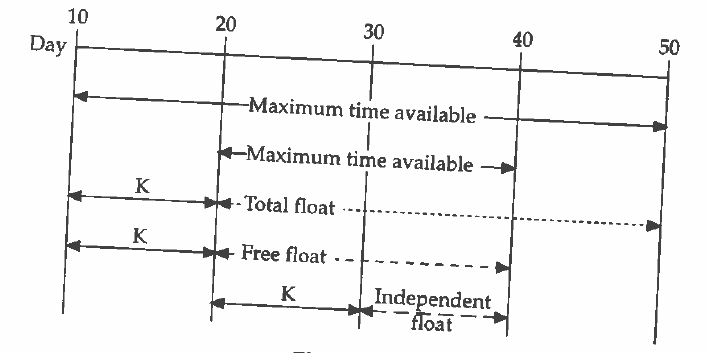
\includegraphics[width=0.4\linewidth]{images4/333-b}
\caption{}
\label{fig:333-b}
\end{figure}


%- 333 
%======================%
Total Float = 50 -10 -10 = 30 days  

\begin{itemize}
	\item b) Free float This is the amount of time an activity can be delayed without affecting the commencement of a subsequent activity at its earliest start time, but may affect float of a previous activity. Free Float = Earliest Head time - Earliest Tail time - Activity Duration Free Float = 40 -10 -10 = 20 days  
	
\item Independent float This is the amount of time an activity can be delayed when all preceding activities are completed as late as possible and all succeeding activities completed as early as possible. Independent float therefore does not affect the float of either preceding or subsequent activities. Independent float = Earliest Head time - Latest Tail time - Activity Duration Independent float = 40 - 20 -10 = 10 days  
	
\item For examination purposes the most important type of float is Total Float because it is involved with the overall project duration. On occasions the term 'Float' is used without qualification. In such cases assume that Total Float is required. 
	
\item The total float can be calculated separately for each activity but it is often useful to find the total float over chains of non-critical activities between critical events. For example in Figure 23/4 the only non-critical chain of activities is C, E for which the following calculation can be made: 
\item 	Non-critical Time Time Total float chain required available over chain C, E 3 + 1 =  7 - 1 = fislaa  = 2 days 
	If some of the 'chain float' is used up on one of the activities in a chain it reduces the leeway available to other activities in the chain. Alternative terms for Earliest Head Time and Latest Headtime are Earliest Finishing Time (EFT) and Latest Finishing Time (LFT), respectively.
	
\end{itemize}
\subsection{Example of float calculations} the example used in the preceding chapter is
 reproduced below with the addition of activity durations. It is required to find the critical path and all floats. 

%- 334 
%======================%
%- Page 335
\begin{center}
\begin{tabular}{|c|c|c|c|}\hline
Activity	&	Preceding	&	Activity	&	Activity	\\
&	Activity	&	Description	&	Duration	\\ \hline
A	&		&	Design Hull	&	9	\\ \hline
B	&		&	Prepare Boat Shed 	&	3	\\ \hline
C 	&	A 	&	Design Mast and Mast Mount 	&	8	\\ \hline
D 	&	A 	&	Obtain Hull 	&	2	\\ \hline
E 	&	A 	&	Design Sails 	&	3	\\ \hline
F 	&	C 	&	Obtain Mast Mount 	&	2	\\ \hline
G 	&	C 	&	Obtain Mast 	&	6	\\ \hline
H 	&	C 	&	Design Rigging 	&	1	\\ \hline
J	&	B, D 	&	Prepare Hull 	&	4	\\ \hline
K	&	F, J	&	Fit Mast Mount to Hull 	&	1	\\ \hline
L 	&	E, H, G, K 	&	Step Mast 	&	2	\\ \hline
M 	&	E,H 	&	Obtain Sails and Rigging 	&	3	\\ \hline
N 	&	L,M 	&	Fit Sails and Rigging 	&	4	\\ \hline
\end{tabular}
\end{center}
\subsection{Solution}
The network is shown in the normal manner in Figure 23/6 from which it will be seen 
that the critical path is: 
Activities A, C, G, L, N with a duration of 29 days. 
\begin{figure}[h!]
\centering
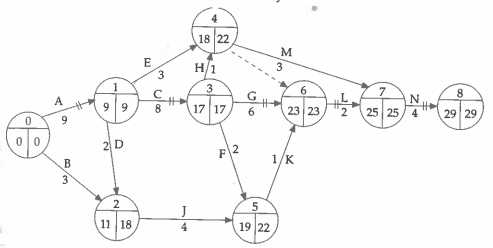
\includegraphics[width=0.4\linewidth]{images4/335-a}
\caption{}
\label{fig:335-a}
\end{figure}

%======================%
A U 9 9 9 
B 0 0 11 18 3 15 8 8 
C 9 9 17 17 8 
D 9 9 11 18 2 7" 
E 9 9 18 22 3 10 6 6 
F 17 17 19 22 2 3 17 17 23 23 6 
H 17 17 18 22 1 4 
J 11 18 19 22 4 7 4 
K 19 22 23 23 1 3 1 
L 23 23 25 25 2 
M 18 22 25 25 3 4 4 
N 25 25 29 29 4 
* Critical activities Float calculations Project XXX. Table 1 The total float on the non critical chains can also be calculated: Non-critical Time Time Total float chain required available over chain l3, J, K 8 23 15 D, J, K 7 14 7 F, K 3 6 3 E, M 6 16 10 H, M 4 8 4 E, dummy 3 14 9 H, dummy 1 6 5 

\subsection{Slack} %- 7. 
This is the difference between the EST and LST for each event. Strictly it does not apply to activities but on occasions the terms are confused in 
examination questions and unless the context makes it abundantly clear that event slack is required, it is likely that some form of activity float is required. 
Events on the critical path have zero slack.
\subsection{Further project time analysis} 
%-8. 
More sophisticated time analysis presupposes that some form of distribution is 
available for each activity time estimate, for example, the three time estimates described in Para 2. These can be used to make statements about the 
probability of achieving scheduled dates. Probability example. Assume that a simple project has the following network shown in Fig 23/7. 
The activity times are in weeks and three estimates have been given for each activity. The expected durations can be found using what is known as 
the PERT formula: Optimistic time + Pessimistic time + 4 x Most likely time 
336 
6 

%- Page 336
%======================%
% Top of Page 337
pendent float FT-LST-D) 
8 
6 

For example: 

Figure 23/7 Critical path (B, D, F) expected duration 4 + 6 + 4(5) B - 6 = 5 weeks 
5.6 + 15 + 4(7) D - 6 - 8.1 weeks 
3 + 5.4 + 4(4.5) F -  6 - AA 
Scheduled date for completion Week 19 
ila If the critical activities were to occur at their optimistic times, event 4 would be reached in 12.6 weeks but if the critical activities occurred at their pessimistic times, event 4 would be reached in 26.4 weeks. As these durations span the scheduled date of week 19 some estimate of the probability of achieving the schedule date must be calculated, as follows. 
a) Make an estimate of the Standard Deviation for each of the critical activities.

 If no additional information is available the following PERT formula can be used. Pessimistic time - Optimistic time 
6 
6 - 4 i.e. Standard Deviation Activity B = —6-- = 0.33 
15 - 5.6 Activity D = 6 = 1.57 
5.4 - 3 Activity F = --7— = 0.4 Find the standard deviation of event 4 by calculating the statistical sum (the square root of the sum of the squares) of the standard deviations of all activities on the critical path. i.e. Standard Deviation of Event 4 = V0.332 + 1.572 + 0.42 = 1.65 weeks 
%- 337 

%=========================%
% Top of Page 338
%- 23 Network analysis - time analysis 
c) Find the number of event standard deviations that the scheduled date is away from 
the expected duration. 
19 -17.5 
i.e.  1.65 - 0.91 
d) Look up this value (0.91) in a table of areas under the Normal Curve to find the prob-
ability (Table I). In this case the probability of achieving the scheduled date of week 
19 is 82%. 
Probability interpretation. If management consider that the probability of 82% is not high 
enough, efforts must be made to reduce the times or the spread of time of activities on the 
critical path. It is an inefficient use of resources to try to make the probability of reaching 
the scheduled date 100\% or very close to 100\%. In this case management may well accept 
the 18\% chance of not achieving the schedule date as realistic. 
\subsubsection{Notes:} 
a) The methods of calculating the Expected Duratio► and Standard Deviation as shown 
above cannot be taken as strictly mathematically valid but are probably accurate 
enough for most purposes. It is considered by some experts that the standard devia-
tion, as calculated above, underestimates the 'true' standard deviation. 
b) When activity times have variations the critical path will often change as the varia-
tions occur. It is necessary therefore to examine critical and near critical activity paths 
when tackling an examination question involving variable activity times. 
\subsection{Discrete probabilities}
9 Instead of the continuous probabilities, which were derived and used in the example in 
Para 7 above, on occasions probabilities are sometimes expressed in discrete terms. For 
example the time estimates for an activity could be given as follows: 
Estimates 
Activity Time Probability 
A 
1 1 
8 weeks 0,61 weeks 0.4 
The expected time for activity A would be (8 x 0.6) + (11 x 0.4) = 9.2 weeks. 
Discrete probability example. Assume that time estimates have been made for the 
following network using discrete probabilities thus: 
338 
Scheduled date 
week 14 
Figure 23/8 


%======================%
date is away from 
ye to find the prob-duled date of week 
y of 82% is not high of activities on the bability of reaching ant may well accept 
23 Network analysis - time analysis Activity A B C Estimates Time (Weeks) Probability [ 6 10 0.5 0  0.5 [ 3 0.4 5 0.6 [ 12 0.6 14 0.3 17 0.1 

\begin{figure}
\centering
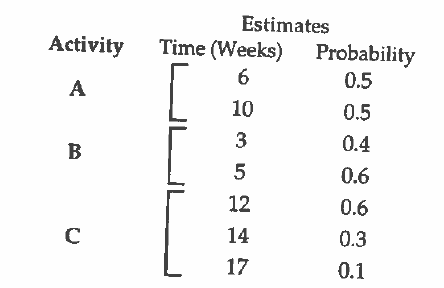
\includegraphics[width=0.4\linewidth]{images4/339-a}
\caption{}
\label{fig:339-a}
\end{figure}


The expected times for the activities are: 
\begin{itemize}
	\item A = (6 x 0.5) + (10 x 0.5) = 8 
	\item B = (3 x 0.4) + ( 5 x 0.6) = 4.2 
	\item C = (12 x 0.6) + (14 x 0.3) + (17 x 0.1) = 13.1 
\end{itemize}

Deviation as shown On the basis of the expected times the critical path is C with a duration of 13.1 weeks. probably accurate However, numerous other possibilities exist and the probabilities of the various comple-the standard devia- tion times and thus of achieving the schedule date of week 14 can be evaluated as ation. follows: hange as the varia- The A, B route can have four durations, each with an associated probability thus: ritical activity paths A, B route y times. 
d in the example in discrete terms. For 
4Rdac been made for th 
late 

Durations 9 11 13 15 weeks Probability 0.2 0.3 0.2 0.3 
(These values are found by combining the durations and probabilities of Activities A and B. For example Activity A duration of 6 weeks, probability 0.5, can be combined with Activity B duration of 3 weeks, probability 0.4, to give 9 weeks duration and probability of 0.2 ( i.e. 0.5 x 0.4). C route 
Duration 12 14 17 weeks Probability 0.6 0.3 0.1 
The A, B route and the C route alternate as the critical path with varying probabilities as shown in the following table. 
\begin{figure}
\centering
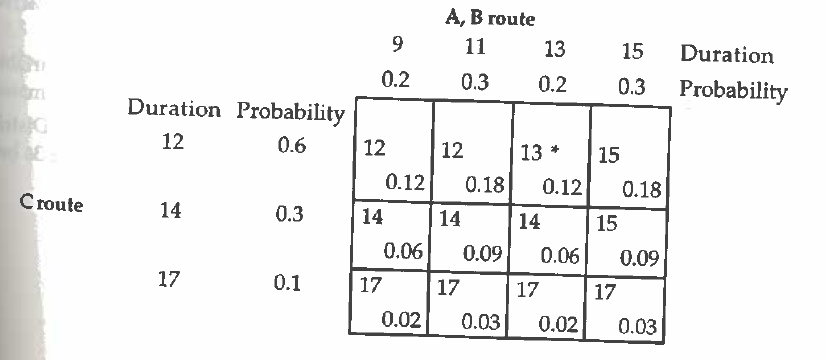
\includegraphics[width=0.4\linewidth]{images4/339-b}
\caption{}
\label{fig:339-b}
\end{figure}

%- 339 
%=================================%
%-Page 340
23 Network analysis — time analysis 
This means that if the A, B route with 13 weeks duration, probability 0.2, occurs at the 
same time as the C route duration of 12 weeks, probability 0.6, the critical path would be 
13 weeks i.e. the longer duration, with the probability of 0.12 (0.6 x 0.2). Summary of possible durations 
12 weeks probability (0.12 + 0.18) = 0.30 
13 weeks probability (0.12) = 0.12 
14 weeks probability (0.06 + 0.09 + 0.06) = 0.21 
15 weeks probability (0.18 + 0.09) = 0.27 
17 weeks probability (0.2 + 0.3 + 0.2 + 0.3) = 0.10 
LOQ Thus the probability of achieving 14 weeks or less is 0.63 (0.30 + 0.12 + 0.21) and the prob-
ability of exceeding the scheduled date is 0.37. 
\subsection{Summary}
10. a) Basic time analysis of a network involves calculating the critical path i.e. the shortest 
time in which the project can be completed. 
b) The critical path is established by calculating the EST (Earliest Start Times) and LST 
(Latest Start Time) for each event and comparing them. The critical path is the chain 
of activities where the EST's and LST's are the same. 
c) Float is the spare time available on non-critical activities. There are three types of 
float; total float, free float and independent float. 
d) To calculate the probability of achieving scheduled dates it is necessary to establish 
what variability is likely to exist for each activity. 
e) Given activity time estimates the expected value of the project duration is calculated 
and an estimate made of the activity standard deviations. 
f) The activity standard deviations are combined to form the standard deviation of the 
overall project so that probability estimates can be made for various project duration 
possibilities. 
\subsection{Points to note}
11. a) The problems of dealing with uncertainty occur again and again in quantitative tech-
niques. Increasingly examination questions are likely to contain variable activity 
times and associated probabilities. 
b) When variable time estimates are used, near criticalpaths may have more variability 
than the critical path so the near critical paths may influence probability estimates. 
c) The basis of the Standard Deviation estimate given in para 8 is the Normal Distribu-
tion. It is known that virtually all of the distribution lies within the mean ± 3s hence 
the formula given 
34O 
max — min 
i.e.   — 
6 
:curs at the 
h would be 
id the Fob- 

%= 23 Network analysis — time analysis 
However the tails of the distribution are unlikely to occur very often so the 95\% 
concept may be used in which case the range becomes mean $\pm 2 \sigma$. If this is thoought to
be realistic the revised formula below can be used.  
\[Pessimistic time — Optimistic time   \]
—a' 
\subsection{Self reviewquestions} Numbers in brackets refer to paragraph numbers 
\begin{enumerate}
	\item What types of time estimates are made for activity durations?(2) 
	\item What is the critical path? (3) 
	\item What are the ESTs and LSTs? (3) 
	\item How is the critical path determined? (4) 
	\item What is float? (5) 
	\item When multiple time estimates of activity durations are availablethow ca 
	the shortest calculated of the probability of completing the network in a given time?n an estimate be 
	(8)
\end{enumerate}
 
\subsection{Exercises with answers} 
?s) and LST 1. Find the critical path of the following network using the EST/LSTs. 
is the chain 
.ee types of 
2 
1 
7 
3 
1 
to establish 
6 
5 
5 
4 
1 
2 
s calculated 
6 3 2 
7 5 3 
ation of the 
8 
2, 6 5 
Id duration 
9 
7, 8 11 
10 
3 7 
11 
4 4 
12 9, 10, 11 3 
itative tech- 

2. Calculate the floats of the network in question 1. 4 
ble activity 3. The standard deviations of the activities on the critical path in question 1 are: 1, 2, 1.5, 3, 
2.5 and 3 respectively q 
Based on these values calculate the probability of achieving a variability ' scheduled time of 40 days for the project duration. 
,stimates. 
Lai Distrib11- 
1 ± 3s herlce 
Activity Preceding activity Duration (days) 
4 
341 
%================%

%- 23 Network analysis - time analysis 
Answers to exercises 1. 

2. Total Free Independent float float float Activity EST LST EFT LFT D LFT - EST - D EFT - EST - D EFT - LST - D 
*1 0 0 4 4 4 2 4 4 11 15 7 *3 4 4 9 9 5 4 4 4 10 22 6 5 11 15 13 21 2 *6 9 9 15 15 3 7 13 21 23 23 5 *8 12 12 23 23 11 *9 23 23 30 30 7 10 9 9 30 30 4 11 10 22 30 30 3 *12 30 30 34 34 4 
3. s.d. of critical path = 412 + 22 + 1.52 + 32 40- 34 :.Z = 5.61 = 1.07 
342 
-4 -12 8 - J.- S 5 ...a - - 17 17 17 17 17 5 - + 2.52 + 32 = 5.61 
From Table 1 the probability is nearly 36% 


%=================%

\end{document}